\documentclass[preprint,12pt]{elsarticle}
\usepackage{xcolor}
\usepackage[colorlinks]{hyperref}
\usepackage{graphicx,amsmath,amssymb,amsthm,marvosym,tikz}
\usepackage{tikz}
\usetikzlibrary{backgrounds}
\usetikzlibrary{patterns,shapes.misc, positioning}

\begin{document}

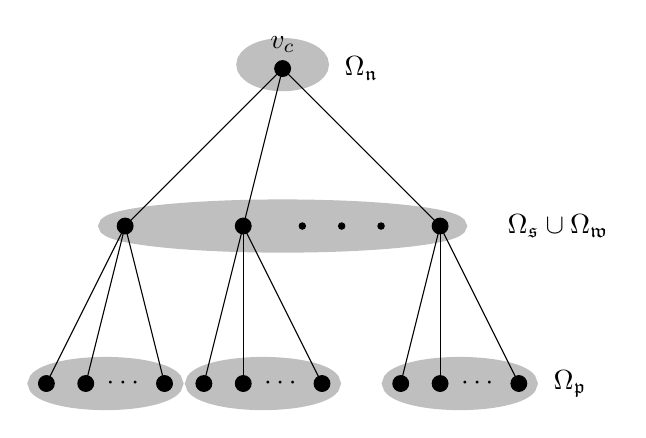
\begin{tikzpicture}[scale=0.5]
   \filldraw[lightgray,line width=5pt,rounded corners=4pt]  (0,0.1) ellipse (1cm and 0.5cm);
    \filldraw[lightgray,line width=5pt,rounded corners=4pt]  (0,-4) ellipse (4.5cm and 0.5cm);
     \filldraw[lightgray,line width=5pt,rounded corners=4pt]  (-4.5,-8) ellipse (1.8cm and 0.5cm);
     \filldraw[lightgray,line width=5pt,rounded corners=4pt]  (-0.5,-8) ellipse (1.8cm and 0.5cm);
     \filldraw[lightgray,line width=5pt,rounded corners=4pt]  (4.5,-8) ellipse (1.8cm and 0.5cm);
    \filldraw[fill=black](0,0) circle (0.2cm);
    \filldraw[fill=black](-4,-4) circle (0.2cm);
    \filldraw[fill=black](-1,-4) circle (0.2cm);
    \filldraw[fill=black](4,-4) circle (0.2cm);
    \filldraw[fill=black](-6,-8) circle (0.2cm);
     \filldraw[fill=black](-5,-8) circle (0.2cm);
      \filldraw[fill=black](-3,-8) circle (0.2cm);
       \filldraw[fill=black](-2,-8) circle (0.2cm);
        \filldraw[fill=black](-1,-8) circle (0.2cm);
         \filldraw[fill=black](1,-8) circle (0.2cm);
          \filldraw[fill=black](6,-8) circle (0.2cm);
           \filldraw[fill=black](3,-8) circle (0.2cm);
            \filldraw[fill=black](4,-8) circle (0.2cm);
            \draw(0,0)--(4,-4);
\draw(0,0)--(-4,-4);
\draw(0,0)--(-1,-4);
\draw(-6,-8)--(-4,-4);
 \draw(-5,-8)--(-4,-4); 
 \draw(-3,-8)--(-4,-4);
 \draw(-2,-8)--(-1,-4);
 \draw(-1,-8)--(-1,-4);
 \draw(1,-8)--(-1,-4);
 \draw(6,-8)--(4,-4);
  \draw(3,-8)--(4,-4);
   \draw(4,-8)--(4,-4);
 \filldraw[fill=black](0.5,-4) circle (0.08cm); 
  \filldraw[fill=black](1.5,-4) circle (0.08cm); 
   \filldraw[fill=black](2.5,-4) circle (0.08cm); 
\node at (-4,-8){$\cdots$};
 \node at (0,-8){$\cdots$}; 
 \node at (5,-8){$\cdots$};
 \node at (0,0.6){$v_c$};
 \node at (2,0){$\Omega_{\mathfrak{n}}$};
 \node at (7,-4){$\Omega_{\mathfrak{s}}\cup \Omega_{\mathfrak{w}}$};
  \node at (7.3,-8){$\Omega_{\mathfrak{p}}$};
\end{tikzpicture}

\end{document}